\documentclass[letterpaper, 10 pt, conference]{ieeeconf}

\usepackage{cite}
\usepackage{graphicx}
\usepackage{amsmath,amsfonts,amssymb}
\usepackage{pgfplots}

\pgfplotsset{compat=1.7}

\graphicspath{ {figures/} }

\renewcommand{\vec}[1]{\boldsymbol{#1}}

\renewcommand{\eqref}[1]{\textup{{\normalfont(\ref{#1}}\normalfont)}}


\title{\textbf{AprilTrack: A Particle-Filter based AprilTag Tracker}}
\author{Daniel Pfrommer}
\date{}

\begin{document}

\maketitle

\begin{abstract}

	The AprilTrack algorithm proposed in this paper seeks to bridge two existing fields of research in computer vision literature: fiducial detection and monocular object tracking. With a rise in the popularity of fiducials, or artificial markers, as a source of ground-truth pose estimation for visual odometry datasets and mobile robots, there has been considerable interest in designing robust and blur-resistant fiducials. Rather than devising a new fiducial, this work attempts to improve on existing fiducials, such as the popular AprilTag marker, by augmenting fiducial detection algorithms with a particle-filter based monocular object tracker which reliably tracks a fiducial's position and orientation in six degrees of freedom, allowing for tag-based localization in situations where current detectors would be unable to do so. This novel patch-based particle filter tracking algorithm, which is extended to simulatenously track multiple tags in ego-motion scenarios, is qualitatively and quantitatively evaluated on several AprilTag sequences, demonstrating that it is capable of reliably localizing blurred tags.
	
\end{abstract}

\section{Introduction}


Visual tracking of fiducial markers (or simply fiducials) plays an important role in many robotics and computer vision related fields and applications, including augmented and virtual reality \cite{AugmentedReality}, visual odometry/SLAM \cite{TagSLAM}, and object tracking. However, as many of these applications involve the use of fiducials in structured indoors environments where illumination is often limited, long exposure times to compensate for the reduced lighting produce blurred images, especially when taken from a mobile platform such as a quadrotor or a handheld device.

The focus of this work is primarily on providing better pose estimation for visual odometry datasets which use AprilTags placed to known locations to provide the ground truth pose data. As the pose estimation in this scenario can be done in a post-processing step after the data has been collected, the current implementation of AprilTrack is not designed to run in realtime. We intend to explore the use of AprilTrack in realtime scenarios in future research.

\subsection{Previous Work}

 The majority of previous literature in fiducial detection has been focused single-frame fiducial detection \cite{RUNETag, BlurResilient, AprilTag}. A common assumption in these algorithms is that the image being processed shows little motion blur, an expectation which breaks down in empirical situations. For instance, the widely-used AprilTag marker \cite{AprilTag} and its successor, the AprilTag 2 \cite{AprilTag_2}, rely on strong gradients between the tag's background and the surrounding white border to detect the tag. As shown in figure \ref{fig:blurred_tag}, oftentimes such algorithms fail to detect tags that have been blurred, either missing them entirely or mistakenly discarding them when eliminating false positives through some encoded fiducial ID (for AprilTags this consists of a 6x6 binary grid in the center of the tag which is used to verify the validity of the detection).

\begin{figure}[b]
	\centering
	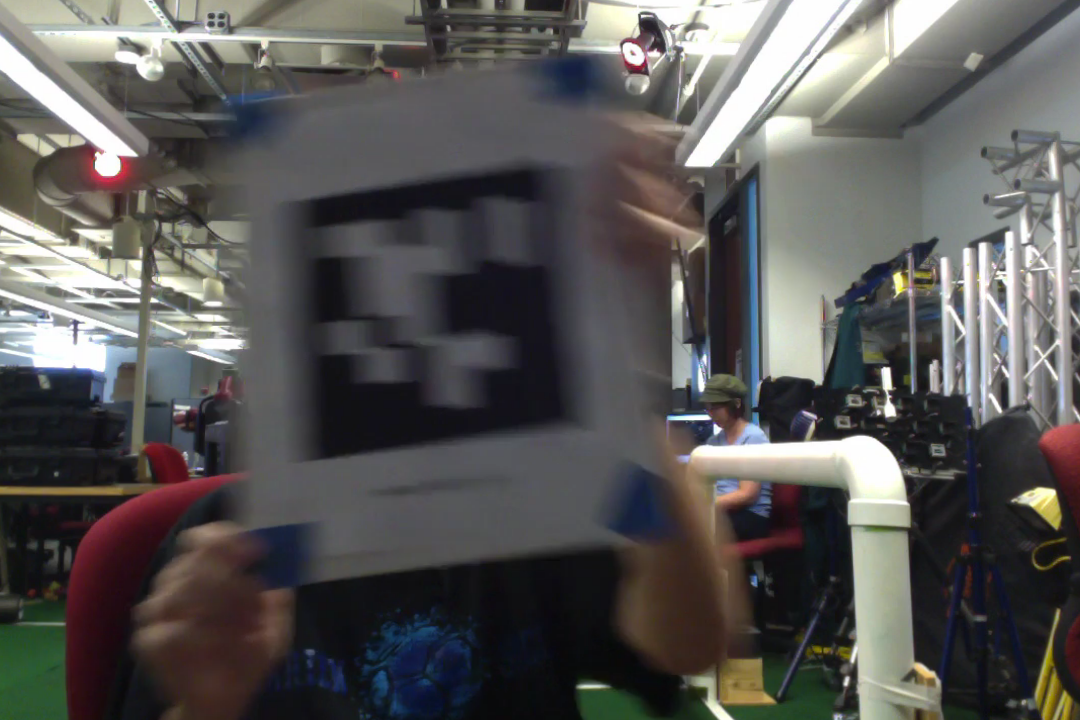
\includegraphics[width=6cm, height=4cm]{blurred_tag}
	\caption{A blurred AprilTag. Such tags are difficult for still frame based algorithms to detect as the payload (the ID encoded in the center of the tag) will cause the tag to be discarded as a false positive.}
	\label{fig:blurred_tag}
\end{figure}

Previously, there has been interest in designing blur resilient fiducials. Meghshyam et al. \cite{BlurResilient} have developed ringed markers to ensure that a region of the tag will always be perpendicular to the blur direction. However, this approach, while resistent to linear blur, does not take into account more complex blurs (e.g resulting from the tag pivoting around the vertical axis). In addition, the increased resilience to blur comes at the cost of localization accuracy as only the center point of the ringed tag can be reliably determined \cite{BlurResilient}, whereas with other fiducials, such as the AprilTag \cite{AprilTag}, full pose estimation in 6 degrees of freedom (DOF) can be done based on just a single tag. Another significant disadvantage of the ringed marker from Meghshyam et al. is the limited number of tag ID's, as their proposed encoding method allows for a maximum of 4 distinct tags \cite{BlurResilient}.


Unlike previous attempts to engineer more resilient tags, the algorithm proposed here exploits the temporal coherence between successive frames in a video sequence to track a tag's location between successful detections. As many high-blur scenarios involve a continuous stream of images taken at equidistant time intervals (e.g a quadroter-mounted moving camera viewing tags or a stationary camera tracking an AprilTag-labeled moving object), we propose to use knowledge of a fiducial's prior location to augment the detection algorithm. As such, this paper presents a novel particle-filter-based tracking algorithm (AprilTrack) capable of tracking AprilTags in 6 DOF with both joint-tag motion and camera ego-motion.
	
Previous work involving the tracking of blurred objects includes the Blur-driven Tracker (BLUT) framework proposed by Wu et al. \cite{BLUT} for tracking motion-blurred targets. BLUT, a particle-filter based tracker, works on the observation that blur strength and direction can be used estimate an object's velocity and provide valuable information for successfully tracking a blurred object. While capable of reliably tracking blurred objects, BLUT suffers from the disadvantage that it can do so only in two dimensions (i.e it is assumed that the object always faces the camera) and so cannot track a sequence of involving arbitrary tag rotations and translations.


The novel method proposed in this paper augments the AprilTag detection algorithm originally designed by Olson \cite{AprilTag} and improved by Wang et al \cite{AprilTag_2} with a particle-filter based algorithm to reliably track an AprilTag through an arbitrary sequence of images, providing valuable fiducial-based position information when existing methods would be unable to do so. In addition, the proposed algorithm is extended to incorporate the joint motion of an arbitrary number of tags to increase the accuracy of the tracked orientation and position.


\textbf{Overview.} The remainder of the paper is organized as follows. Section 2 gives an overview of the method proposed in this paper and describes the algorithm in detail. Section 3 describes the implementation of the algorithm and evaluates its performance on a manually-labeled dataset of blurred moving tags both quantitatively and qualitatively. In section 4 we discuss the limitations of this approach and suggest possible avenues of future research.

\section{Method}

The AprilTrack algorithm is similar in concept to the BLUT tracker by Wu et al. \cite{BLUT} in that it uses a particle filter to integrate all available information about a marker's position. Overall, the description of the algorithm can be broken down into three parts: one describing the particle filter, another on the method for evaluating candidate particles, and one describing the modifications made to simulatenously track multiple tags.

\subsection{The Particle Filter}

The particle filter used for the AprilTrack algorithm is a Bayesian Sequential Importance Resampling (SIR) technique which approximates a posterior distribution of state variables at discrete time intervals. There are three major steps in the algorithm: prediction, update, and resampling. We use the vector  $\vec{x}_t$  to denote the 13 dimensional state vector describing the position, orientation, velocity, and rotational velocity of the tracked target at time $t$ 

\begin{equation}
\vec{x}_t = 
\begin{bmatrix}
	\vec{r} \\
	\dot{\vec{r}} \\
	\vec{q} \\
	\vec{\omega}
\end{bmatrix}
\end{equation}

where $\vec{r}$ is the three dimensional position of the tracked object, $\dot{\vec{r}}$ is the three dimensional velocity, $\vec{q}$ is a four dimensional unit quaternion containing the pose of the tracked object, and $\vec{\omega}$ is an angular velocity with components $\omega_x$, $\omega_y$, and $\omega_z$.




\textbf{Optimal filtering.} The prediction step can be formulated in a Bayesian setting as the computation of the prior distribution $p(\vec{x}_{t}|\vec{z}_{t-1})$ from the filtering distribution $p(\vec{x}_{t-1}|\vec{z}_{1:t-1})$ where $\vec{z}_t$ represents the measurement (appearance of a fiducial) taken at time $t$. As in \cite{ParticleNotes}:

\begin{equation} \label{eq:predict}
p(\vec{x}_t|\vec{z}_{1:t-1}) = \int p(\vec{x}_t | \vec{x}_{t-1})p(\vec{x}_{t-1}|\vec{z}_{1:t-1})d\vec{x}_{t-1}
\end{equation}

Likewise, the update step can be formulated in a similar manner, where the prior distribution calculated in the prediction step is updated with the latest measurement to obtain the posterior over $\vec{x}_t$. Mathematically this can be derived using Bayes' law to express $p(\vec{x}_t|\vec{z}_{1:t})$ in terms of $p(\vec{z}_t|\vec{x}_t)$ and $p(\vec{x}_t|\vec{z}_{1:t-1})$. Using Bayes' law yields
\begin{equation*}
	p(\vec{x}_t|\vec{z}_{1:t}) = p(\vec{x}_t|\vec{z}_t,\vec{z}_{1:t-1})
\end{equation*}
\begin{equation*}
p(\vec{x}_t|\vec{z}_t,\vec{z}_{1:t-1}) = \frac{p(\vec{z}_t|\vec{x}_t, \vec{z}_{1:t-1})p(\vec{x}_t|\vec{z}_{1:t-1})p(\vec{z}_{1:t-1})}{p(\vec{z}_{1:t})}
\end{equation*}
As the model $p(\vec{x}_t|\vec{x}_{t-1})$ is Markovian, the current measurement is conditionally independent of previous measurements given $\vec{x}_t$, meaning that $p(\vec{z}_{t}|\vec{x}_t, \vec{z}_{1:t-1})$ can be written as $p(\vec{z}_t|\vec{x}_t)$. $p(\vec{z}_{1:t})$ can also be expressed as $p(\vec{z}_t|\vec{z}_{1:t-1})p(\vec{z}_{1:t-1})$ resulting in the final update equation \cite{ParticleNotes}
\begin{equation} \label{eq:update}
	p(\vec{x}_t|\vec{z}_{1:t}) = \frac{p(\vec{z}_{t}|\vec{x}_t)p(\vec{x}_{t}|\vec{z}_{1:t-1})}{p(\vec{z}_t|\vec{z}_{1:t-1})}
\end{equation}





\textbf{Particle Filters.} In this regard, particle filters attempt to approximate the posterior distribution at time $t-1$, $p(\vec{x}_{0:t-1}|\vec{z}_{1:t-1})$, using Monte-Carlo methods. A particle filter consists of a set of $N$ samples $\{ (\vec{x}^i_{t-1}, w^i_{t-1}) \}_{i=1}^N$ drawn from the proposal distribution $q(\vec{x}^i)$ where each sample is called a \emph{particle}. This allows for the filtering distribution $p(\vec{x}_{0:t-1}|\vec{z}_{1:t-1})$ to be approximated by (as described in \cite{ParticleNotes})

\begin{equation}
 	p(\vec{x}_{0:t-1}|\vec{z}_{1:t-1}) \approx \sum_{i=1}^{N}{w^i_{t-1}\delta_{\vec{x}^i_{0:t-1}}}
\end{equation}

 where
\begin{equation}
	\sum_{i=1}^{N}{w^i_t} = 1
\end{equation}


As the particles are drawn from the proposal distribution $q(\vec{x})$, the sample weight $w^i$ must take into account any discrepancy between $p(\vec{x})$ and $q(\vec{x})$ so that $w^i_t \propto p(\vec{x}^i_{1:t}|\vec{z}_{1:t})/q(\vec{x}^i_{1:t}|\vec{z}_{1:t})$.

In the simplified case of a Sequential Importance Resampling algorithm, the prediction and update equations derived from \eqref{eq:predict} and \eqref{eq:update} can, in the context of a SIR particle filter, be simplified to:

\begin{equation}
	\vec{x}^i_t \sim p(\vec{x}_t|\vec{x}^i_{t-1})
\end{equation}

\begin{equation}
	w \propto p(\vec{z}_t|\vec{x}^i_t)
\end{equation}
where $\vec{x}^i_t \sim p(\vec{x}_t|\vec{x}^i_{t-1})$ denotes that, during the prediction step, the particles for the prior distribution at time $t$ are sampled from the known distribution $p(\vec{x}_t|\vec{x}^i_{t-1})$. The distribution $p(\vec{z}_t|\vec{x}^i_t)$ for updating particle weights will be defined in section \ref{sec:candidate_particles}.

In AprilTrack, we model $p(\vec{x}_t|\vec{x}^i_{t-1})$ as a multivariate gaussian distribution with standard deviation $\vec{\sigma}$ around a mean $\vec{\mu}$ where
\begin{equation} \label{eq:propagation_mean}
\vec{\mu} = 
\begin{bmatrix} 
	\vec{r}^i_{t-1} + \Delta t \dot{\vec{r}}^i_{t-1} \\
 	\dot{\vec{r}}^i_{t-1} \\
	\vec{q}^i_{t-1} \dot{\vec{q}}^i_{t-1}\\
	\vec{\omega}^i_{t-1}
\end{bmatrix}
\end{equation}

In equation \eqref{eq:propagation_mean}, $\Delta t$ is the elapsed time and $\dot{\vec{q}}^i_{t-1}$ is the quaternion representation of $\Delta t  \vec{\omega}^i_{k-1}$, as described in \cite{KalmanFilter}. We also use the \emph{noise quaternion} formulated in \cite{KalmanFilter} to apply the gaussian noise to the quaternion $\vec{q}^i_{k-1} \dot{\vec{q}}^i_{k-1}$. For simplicity, we make the assumption that the input images have been taken at equidistant time intervals and incorporate $\Delta t$ into the $\vec{\omega}$ and $\dot{\vec{r}}$ components of $\vec{\sigma}$.


After completing the update prediction and update steps and selecting the particle with the highest weight as the most likely candidate, the final resampling step simply consists of drawing a new set of $N$ particles with equal weights (normalized to a total of one) from the distribution $p(\vec{x}_t|\vec{z}_{1:t})$ where $p(\vec{x}_t|\vec{z}_{1:t})$ is approximated by the set of weighted particles.

\begin{equation}
	p(\vec{x}_t|\vec{z}_{1:t}) \approx \sum_{i=1}^{N}{w^i_t\delta_{\vec{x}^i_t}}
\end{equation}

\subsection{Evaluation of Candidate Particles} \label{sec:candidate_particles}

The tracking of AprilTags in 6 DOF requires a method for evaluating the likelihood of candidate particles at arbitrary three dimensional positions and rotations, or $p(\vec{z}_t|\vec{x}^i_t)$. To this effect, the proposed method uses homographies to generate image \emph{patches}, which are unprojected representations of an AprilTag for a particular pose and image.


Given the function $I(\begin{bmatrix} \lambda x, & \lambda y, & \lambda \end{bmatrix}^\intercal )$ representing the intensity of pixel at a particular $(x,y)$ of an image, a patch in the image can be defined by the function 

\begin{equation}
P(x_p,y_p| \vec{H}, I ) = I(\vec{H}  \begin{bmatrix} x_p & y_p & 1\end{bmatrix}^\intercal)
\end{equation}

where $x_p$ and $y_p$ are between $-1$ and $1$ and $\vec{H}$ is a 3x3 matrix (a homography) mapping from $(x_p, y_p, 1)$ to $(\lambda x, \lambda y, \lambda)$ which incorporates the pose of an AprilTag relative to the camera. 


This allows for the evaluation of candidate particle $\vec{x}^i$ by the measuring the similarity between the particle's patch $P^i(x_p,y_p|\vec{H}^i,I)$ in the current image and the patch from the AprilTag's last successful detection, $P_{ref}(x_p,y_p|\vec{H}_{ref},I_{ref})$. Here, $H^i$ can be calculated with

\begin{equation} \label{eq:particle_homography}
\vec{H}^i = \begin{bmatrix}
		\widehat{\vec{q}^i} & \vec{r}^i
	\end{bmatrix} \begin{bmatrix}
		\tau/2 & 0 & 0 \\
		0 & \tau/2 & 0 \\
		0 & 0 & 0 \\
		0 & 0 & 1
	\end{bmatrix}
\end{equation}



where $\widehat{\vec{q}^i}$ is the rotation matrix representation of particle $\vec{x}^i$'s rotation quaternion $\vec{q}$, $\vec{r}$ is the particle's translation, and $\tau$ is the tag's edge length. The patch for the detected AprilTag uses the homography $\vec{H}_{ref}$ supplied by the AprilTag library, which computes the homography using the Direct Linear Transform algorithm \cite{AprilTag}. 


To compare the patches efficiently, $P^i$ and $P_{ref}$ are evaluated at a regular grid from $(-1, -1)$ to $(1, 1)$ at intervals of $2 / \rho$. This results in two $\rho \times \rho$ matrices $\vec{M}^i$ and $\vec{M}_{ref}$. To compare the patches, the error between the two  matrices is calculated using the correlation coefficient between the individual elements of the matrices.

\begin{equation}
	\epsilon(\vec{A}, \vec{B}) = \frac{1}{2} - \frac{\sum_{i=1}^{\rho} \sum_{j=1}^{\rho} (\vec{A}_{ij} - \mu_{\vec{A}})(\vec{B}_{ij} - \mu_{\vec{B}}) }{2\sigma_{A} \sigma_{B}}
\end{equation}

where $\vec{A}$ and $\vec{B}$ are the matrix approximations of two patches, $\sigma_{\vec{A}}$ and $\sigma_{\vec{B}}$ are the standard deviations of the respective matrices' elements and $\mu_{\vec{A}}$ and $\mu_{\vec{B}}$ are their means. By normalizing by mean and standard deviation, using correlation as a similarity metric (as opposed to the sum of the absolute difference or squared difference) ensures lighting invariance for comparing patches containing the same marker under different illuminations.


As in BLUT \cite{BLUT}, the patch error $\epsilon(\vec{M}^{i}, \vec{M}_{ref})$ is used to compute the observation likelihood $p(\vec{z}_t|\vec{x}^i_t)$ to update the weights and select the best particle with


\begin{equation}
	p(\vec{z}_t|\vec{x}^i_t) = exp(-\gamma \epsilon(\vec{M}^i, \vec{M}_{ref}))
\end{equation}

where the parameter $\gamma$ allows for more or less selective resampling.


\begin{figure}[b]
	\centering
	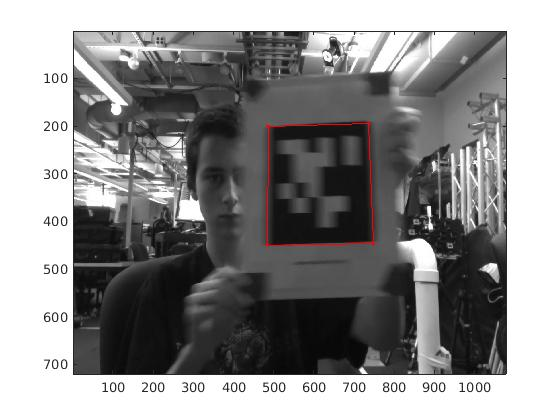
\includegraphics[width=7.5cm,height=5cm]{tracked_tag}
	\caption{A blurred tag being tracked. The red border indicates that the tag was not detected with the AprilTag detector.}
\end{figure}

\begin{figure*}[t]
	\centering
	\label{fig:error}
	\begin{tikzpicture}[trim axis left]
	\begin{axis}[
		width=\textwidth,
		height=9cm,
		title= {Average Corner Error on the Single-Tag Sequence},
		xlabel = {Time (Frame Number)},
		ylabel = {Average Corner Error (Pixels)},
		xmin=0, xmax=250,
		ymin=0, ymax=80,
		xtick={0,50,100,150,200,250},
		ytick={0,10,20,30,40,50,60, 70}
	]
	\addplot [
		color=blue,
		mark=none,
	] table {corner_error.dat};
\end{axis}
\end{tikzpicture}
	\caption{The average corner error between the hand-marked tag location and the tracked location. Much of the error comes from discrepancy between the tracker and the ground truth on the boundaries of the blurred tags. At around frames 30 and 200, the tracker loses the tag momentarily due to a sudden rotation but is able to recover without needing to be manually reset.}
\end{figure*}




\subsection{Multi-Tag Scenarios}

To adapt this method to multi-tag scenarios, several extra parameters have to be introduced. In order to jointly track multiple tags, it is assumed that the relative poses of the tags are known. For each tag $T_k$ with ID $k$, the location $\vec{x}_{k}$ and orientation quaternion $\vec{g}_{k}$ are expressed such that

\begin{equation}
	\vec{X}_c = \widehat{\vec{q}^i} (\widehat{\vec{g}_k} \vec{X}_t + \vec{x}_k) + \vec{r}^i
\end{equation}
where $\vec{X}_t$ is a coordinate relative to the tag's reference frame, $\vec{X}_c$ is relative to the camera reference frame, and $\vec{q}^i$ and $\vec{r}^i$ are the position and orientation of particle $\vec{x}^i_t$. In the simple case of jointly moving tags, the $\vec{H}^i$ from equation \eqref{eq:particle_homography} can then be rewritten as


\begin{equation}
	\vec{H}^i_{k} =
	\begin{bmatrix}
		\widehat{\vec{q}^i \vec{g_k}} & \widehat{\vec{q}} \vec{x_k} + \vec{r}^i
	\end{bmatrix}\begin{bmatrix}
		\tau_k/2 & 0 & 0 \\
		0 & \tau_k/2 & 0 \\
		0 & 0 & 0 \\
		0 & 0 & 1
	\end{bmatrix}
\end{equation}

where $\vec{H}^i_k$ represents the homography for particle $i$ and tag $k$ and $\tau_k$ is the edge length of tag $k$.


In the ego-motion scenario, each particle's rotation and translation can be taken to be the camera's rotation and  translation such that

\begin{equation}
	\widehat{\vec{q}^i}\vec{X}_c + \vec{r}^i = \widehat{\vec{g}_k} \vec{X}_t + \vec{x}_k
\end{equation}

resulting in the homography $\vec{H}^i_k$ and the corresponding patch approximation $\vec{M}^i_k$ where

\begin{equation}
	\vec{H}^i_k = \begin{bmatrix}
		\widehat{\vec{q}^i}^{-1} \widehat{\vec{g}_k} & \widehat{\vec{q}^i}^{-1} (\vec{x}_k - \vec{r}^i)
	\end{bmatrix} \begin{bmatrix}
		\tau_k/2 & 0 & 0 \\
		0 & \tau_k/2 & 0 \\
		0 & 0 & 0 \\
		0 & 0 & 1
	\end{bmatrix}
\end{equation}


In both ego-motion and joint tag motion, the observation likelihood $p(\vec{z}_t|\vec{x}_{t})$ then becomes

\begin{equation}
	p(\vec{z}_t|\vec{x}^i_{t}) = exp(\sum^{K}_{k=1} -\gamma \epsilon(\vec{M}^i_k, \vec{M}_{k, ref}))
\end{equation}

where $K$ is the number of tags being tracked and $\vec{M}_{k,ref}$ is the reference patch approximation for tag $k$ from the last successful detection.



\begin{figure}
	\centering
	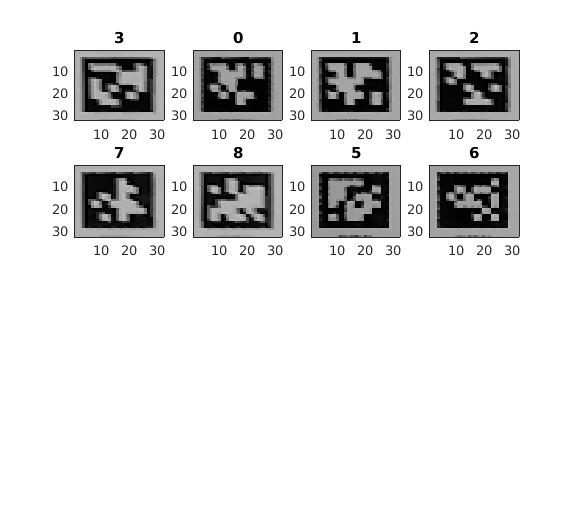
\includegraphics[width=7cm,height=4.75cm]{RefPatches}
	\caption{The reference patches of various tags (by ID) in a multi-Tag tracking scenario.}
\end{figure}
\begin{figure}
	\centering
	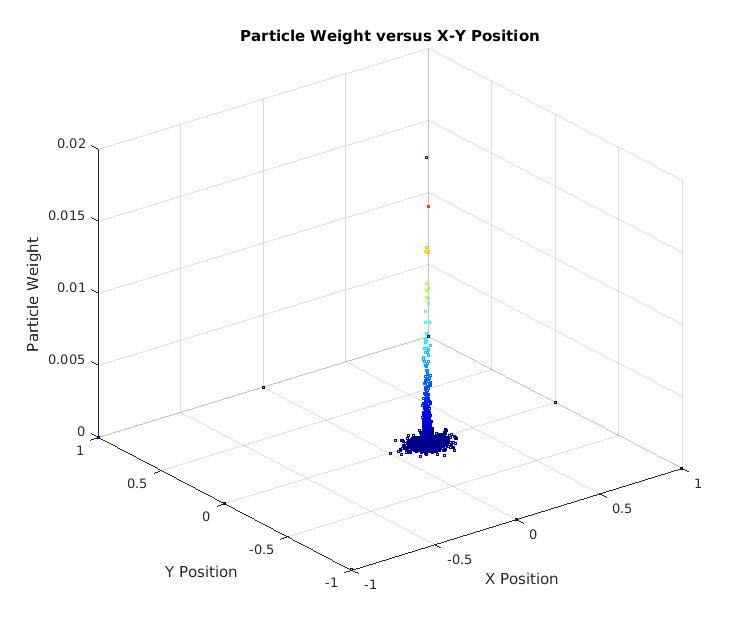
\includegraphics[width=8cm,height=6cm]{Particles2}
	\caption{The distribution of particles and their weights with respect to the X,Y position of the particles.}
\end{figure}

\section{Results and Discussion}

The AprilTrack algorithm was primarily evluated on a manually-labeled single-tag sequence with a moving tag. The algorithm was also run on an ego-motion multi-tag sequence which will be qualitatively discussed.
\footnote{Videos of the sequences and the tracker's performance are available online at https://www.youtube.com/watch?v=kV8z3st9rlk and https://www.youtube.com/watch?v= }


The specific implementation of the AprilTrack algorithm used in this experiment was written in MATLAB. For both scenarios, the parameters $\gamma = 10$, $\rho=32$ were used. $\tau$ was $0.1936$ m for all tags, slightly larger than the actual tag size of $0.1635$ m to include some of the whitespace around the tag. In the single-tag scenario, the standard deviation $\vec{\sigma}$  of the gaussian noise used in the state transition distribution $p(\vec{x}_t|\vec{x}^i_{t-1})$ was $0.01$ for the $\vec{r}$ component, $0.05$ for $\vec{q}$, $0.02$ for $\dot{\vec{r}}$, and $0$ for $\omega$.


When evaluated on the single-tag sequence, the algorithm ran with $N=3000$ at around $1$ fps on an i7 Haswell Intel CPU. In experiments with fewer particles, it was found that the algorithm could track a tag well with as few as $1000$ particles with around $5$ fps. With a more optimized C++ implementation, the framerate could perhaps be brought up to $10-15$ fps, making the algorithm (run with less agressive parameters) a possible candidate for real-time scenarios. Currently, the MATLAB implementation is intended for offline post-processing of a sequence and so real-time performance was not a focus of this research.


As shown in figure \ref{fig:error}, the pixel corner error hovers at around 10 pixels for most of the sequence. The tracker loses the tag momentarily around frames 30 and 200 but is able to recover rapidly without any manual intervention. Much of the error observed throughout the sequence is the result of disagreement on the boundary of a blurred tag rather than a systematic issue with the tracker itself.

When running with a multi-tag configuration, the tracker is able to make use of the additional information to more accurately track the camera's location than in a single-tag scenario. The main challenge for running the algorithm with multiple tags was not successfully tracking the tags---the algorithm was able to do that with half the particles of the single-tag scenario. Rather, the majority of the reprojection error arises from error in the relative tag positions. This opens up new potential avenues of research, such as tag-based bundle adjustment, to alleviate these issues.

\section{Conclusion}

This paper has presented the AprilTrack algorithm augmenting the standard AprilTag detection algorithm with a novel tracker capable of tracking the tags in 6 DOF by using homographies to evaluate candidate particles. Experimental results show that the tracker is capable of accurately tracking both single tags and consolidating information from multiple tags in ego-motion and joint tag-motion scenarios. In future research we plan to investigate other possible error metrics for patch comparison and look to deploy AprilTrack in realtime scenarios.

\bibliographystyle{unsrt}
\bibliography{paper_bib}{}

\end{document}
